\documentclass{report}

%%%%%%%%%%%%%%%%%%%%%%%%%%%%%%%%%
% PACKAGE IMPORTS
%%%%%%%%%%%%%%%%%%%%%%%%%%%%%%%%%


\usepackage[tmargin=2cm,rmargin=1in,lmargin=1in,margin=0.85in,bmargin=2cm,footskip=.2in]{geometry}
\usepackage{amsmath,amsfonts,amsthm,amssymb,mathtools}
\usepackage[varbb]{newpxmath}
\usepackage{xfrac}
\usepackage[makeroom]{cancel}
\usepackage{mathtools}
\usepackage{bookmark}
\usepackage{enumitem}
\usepackage{hyperref,theoremref}
\hypersetup{
	pdftitle={Assignment},
	colorlinks=true, linkcolor=doc!90,
	bookmarksnumbered=true,
	bookmarksopen=true
}
\usepackage[most,many,breakable]{tcolorbox}
\usepackage{xcolor}
\usepackage{varwidth}
\usepackage{varwidth}
\usepackage{etoolbox}
%\usepackage{authblk}
\usepackage{nameref}
\usepackage{multicol,array}
\usepackage{tikz-cd}
\usepackage[ruled,vlined,linesnumbered]{algorithm2e}
\usepackage{comment} % enables the use of multi-line comments (\ifx \fi) 
\usepackage{import}
\usepackage{xifthen}
\usepackage{pdfpages}
\usepackage{transparent}

\newcommand\mycommfont[1]{\footnotesize\ttfamily\textcolor{blue}{#1}}
\SetCommentSty{mycommfont}
\newcommand{\incfig}[1]{%
    \def\svgwidth{\columnwidth}
    \import{./figures/}{#1.pdf_tex}
}

\usepackage{tikzsymbols}
\renewcommand\qedsymbol{$\Laughey$}


%\usepackage{import}
%\usepackage{xifthen}
%\usepackage{pdfpages}
%\usepackage{transparent}


%%%%%%%%%%%%%%%%%%%%%%%%%%%%%%
% SELF MADE COLORS
%%%%%%%%%%%%%%%%%%%%%%%%%%%%%%



\definecolor{myg}{RGB}{56, 140, 70}
\definecolor{myb}{RGB}{45, 111, 177}
\definecolor{myr}{RGB}{199, 68, 64}
\definecolor{mytheorembg}{HTML}{F2F2F9}
\definecolor{mytheoremfr}{HTML}{00007B}
\definecolor{mylenmabg}{HTML}{FFFAF8}
\definecolor{mylenmafr}{HTML}{983b0f}
\definecolor{mypropbg}{HTML}{f2fbfc}
\definecolor{mypropfr}{HTML}{191971}
\definecolor{myexamplebg}{HTML}{F2FBF8}
\definecolor{myexamplefr}{HTML}{88D6D1}
\definecolor{myexampleti}{HTML}{2A7F7F}
\definecolor{mydefinitbg}{HTML}{E5E5FF}
\definecolor{mydefinitfr}{HTML}{3F3FA3}
\definecolor{notesgreen}{RGB}{0,162,0}
\definecolor{myp}{RGB}{197, 92, 212}
\definecolor{mygr}{HTML}{2C3338}
\definecolor{myred}{RGB}{127,0,0}
\definecolor{myyellow}{RGB}{169,121,69}
\definecolor{myexercisebg}{HTML}{F2FBF8}
\definecolor{myexercisefg}{HTML}{88D6D1}


%%%%%%%%%%%%%%%%%%%%%%%%%%%%
% TCOLORBOX SETUPS
%%%%%%%%%%%%%%%%%%%%%%%%%%%%

\setlength{\parindent}{1cm}
%================================
% THEOREM BOX
%================================

\tcbuselibrary{theorems,skins,hooks}
\newtcbtheorem[number within=section]{Theorem}{Theorem}
{%
	enhanced,
	breakable,
	colback = mytheorembg,
	frame hidden,
	boxrule = 0sp,
	borderline west = {2pt}{0pt}{mytheoremfr},
	sharp corners,
	detach title,
	before upper = \tcbtitle\par\smallskip,
	coltitle = mytheoremfr,
	fonttitle = \bfseries\sffamily,
	description font = \mdseries,
	separator sign none,
	segmentation style={solid, mytheoremfr},
}
{th}

\tcbuselibrary{theorems,skins,hooks}
\newtcbtheorem[number within=chapter]{theorem}{Theorem}
{%
	enhanced,
	breakable,
	colback = mytheorembg,
	frame hidden,
	boxrule = 0sp,
	borderline west = {2pt}{0pt}{mytheoremfr},
	sharp corners,
	detach title,
	before upper = \tcbtitle\par\smallskip,
	coltitle = mytheoremfr,
	fonttitle = \bfseries\sffamily,
	description font = \mdseries,
	separator sign none,
	segmentation style={solid, mytheoremfr},
}
{th}


\tcbuselibrary{theorems,skins,hooks}
\newtcolorbox{Theoremcon}
{%
	enhanced
	,breakable
	,colback = mytheorembg
	,frame hidden
	,boxrule = 0sp
	,borderline west = {2pt}{0pt}{mytheoremfr}
	,sharp corners
	,description font = \mdseries
	,separator sign none
}

%================================
% Corollery
%================================
\tcbuselibrary{theorems,skins,hooks}
\newtcbtheorem[number within=section]{Corollary}{Corollary}
{%
	enhanced
	,breakable
	,colback = myp!10
	,frame hidden
	,boxrule = 0sp
	,borderline west = {2pt}{0pt}{myp!85!black}
	,sharp corners
	,detach title
	,before upper = \tcbtitle\par\smallskip
	,coltitle = myp!85!black
	,fonttitle = \bfseries\sffamily
	,description font = \mdseries
	,separator sign none
	,segmentation style={solid, myp!85!black}
}
{th}
\tcbuselibrary{theorems,skins,hooks}
\newtcbtheorem[number within=chapter]{corollary}{Corollary}
{%
	enhanced
	,breakable
	,colback = myp!10
	,frame hidden
	,boxrule = 0sp
	,borderline west = {2pt}{0pt}{myp!85!black}
	,sharp corners
	,detach title
	,before upper = \tcbtitle\par\smallskip
	,coltitle = myp!85!black
	,fonttitle = \bfseries\sffamily
	,description font = \mdseries
	,separator sign none
	,segmentation style={solid, myp!85!black}
}
{th}


%================================
% LENMA
%================================

\tcbuselibrary{theorems,skins,hooks}
\newtcbtheorem[number within=section]{Lenma}{Lenma}
{%
	enhanced,
	breakable,
	colback = mylenmabg,
	frame hidden,
	boxrule = 0sp,
	borderline west = {2pt}{0pt}{mylenmafr},
	sharp corners,
	detach title,
	before upper = \tcbtitle\par\smallskip,
	coltitle = mylenmafr,
	fonttitle = \bfseries\sffamily,
	description font = \mdseries,
	separator sign none,
	segmentation style={solid, mylenmafr},
}
{th}

\tcbuselibrary{theorems,skins,hooks}
\newtcbtheorem[number within=chapter]{lenma}{Lenma}
{%
	enhanced,
	breakable,
	colback = mylenmabg,
	frame hidden,
	boxrule = 0sp,
	borderline west = {2pt}{0pt}{mylenmafr},
	sharp corners,
	detach title,
	before upper = \tcbtitle\par\smallskip,
	coltitle = mylenmafr,
	fonttitle = \bfseries\sffamily,
	description font = \mdseries,
	separator sign none,
	segmentation style={solid, mylenmafr},
}
{th}


%================================
% PROPOSITION
%================================

\tcbuselibrary{theorems,skins,hooks}
\newtcbtheorem[number within=section]{Prop}{Proposition}
{%
	enhanced,
	breakable,
	colback = mypropbg,
	frame hidden,
	boxrule = 0sp,
	borderline west = {2pt}{0pt}{mypropfr},
	sharp corners,
	detach title,
	before upper = \tcbtitle\par\smallskip,
	coltitle = mypropfr,
	fonttitle = \bfseries\sffamily,
	description font = \mdseries,
	separator sign none,
	segmentation style={solid, mypropfr},
}
{th}

\tcbuselibrary{theorems,skins,hooks}
\newtcbtheorem[number within=chapter]{prop}{Proposition}
{%
	enhanced,
	breakable,
	colback = mypropbg,
	frame hidden,
	boxrule = 0sp,
	borderline west = {2pt}{0pt}{mypropfr},
	sharp corners,
	detach title,
	before upper = \tcbtitle\par\smallskip,
	coltitle = mypropfr,
	fonttitle = \bfseries\sffamily,
	description font = \mdseries,
	separator sign none,
	segmentation style={solid, mypropfr},
}
{th}


%================================
% CLAIM
%================================

\tcbuselibrary{theorems,skins,hooks}
\newtcbtheorem[number within=section]{claim}{Claim}
{%
	enhanced
	,breakable
	,colback = myg!10
	,frame hidden
	,boxrule = 0sp
	,borderline west = {2pt}{0pt}{myg}
	,sharp corners
	,detach title
	,before upper = \tcbtitle\par\smallskip
	,coltitle = myg!85!black
	,fonttitle = \bfseries\sffamily
	,description font = \mdseries
	,separator sign none
	,segmentation style={solid, myg!85!black}
}
{th}



%================================
% Exercise
%================================

\tcbuselibrary{theorems,skins,hooks}
\newtcbtheorem[number within=section]{Exercise}{Exercise}
{%
	enhanced,
	breakable,
	colback = myexercisebg,
	frame hidden,
	boxrule = 0sp,
	borderline west = {2pt}{0pt}{myexercisefg},
	sharp corners,
	detach title,
	before upper = \tcbtitle\par\smallskip,
	coltitle = myexercisefg,
	fonttitle = \bfseries\sffamily,
	description font = \mdseries,
	separator sign none,
	segmentation style={solid, myexercisefg},
}
{th}

\tcbuselibrary{theorems,skins,hooks}
\newtcbtheorem[number within=chapter]{exercise}{Exercise}
{%
	enhanced,
	breakable,
	colback = myexercisebg,
	frame hidden,
	boxrule = 0sp,
	borderline west = {2pt}{0pt}{myexercisefg},
	sharp corners,
	detach title,
	before upper = \tcbtitle\par\smallskip,
	coltitle = myexercisefg,
	fonttitle = \bfseries\sffamily,
	description font = \mdseries,
	separator sign none,
	segmentation style={solid, myexercisefg},
}
{th}

%================================
% EXAMPLE BOX
%================================

\newtcbtheorem[number within=section]{Example}{Example}
{%
	colback = myexamplebg
	,breakable
	,colframe = myexamplefr
	,coltitle = myexampleti
	,boxrule = 1pt
	,sharp corners
	,detach title
	,before upper=\tcbtitle\par\smallskip
	,fonttitle = \bfseries
	,description font = \mdseries
	,separator sign none
	,description delimiters parenthesis
}
{ex}

\newtcbtheorem[number within=chapter]{example}{Example}
{%
	colback = myexamplebg
	,breakable
	,colframe = myexamplefr
	,coltitle = myexampleti
	,boxrule = 1pt
	,sharp corners
	,detach title
	,before upper=\tcbtitle\par\smallskip
	,fonttitle = \bfseries
	,description font = \mdseries
	,separator sign none
	,description delimiters parenthesis
}
{ex}

%================================
% DEFINITION BOX
%================================

\newtcbtheorem[number within=section]{Definition}{Definition}{enhanced,
	before skip=2mm,after skip=2mm, colback=red!5,colframe=red!80!black,boxrule=0.5mm,
	attach boxed title to top left={xshift=1cm,yshift*=1mm-\tcboxedtitleheight}, varwidth boxed title*=-3cm,
	boxed title style={frame code={
					\path[fill=tcbcolback]
					([yshift=-1mm,xshift=-1mm]frame.north west)
					arc[start angle=0,end angle=180,radius=1mm]
					([yshift=-1mm,xshift=1mm]frame.north east)
					arc[start angle=180,end angle=0,radius=1mm];
					\path[left color=tcbcolback!60!black,right color=tcbcolback!60!black,
						middle color=tcbcolback!80!black]
					([xshift=-2mm]frame.north west) -- ([xshift=2mm]frame.north east)
					[rounded corners=1mm]-- ([xshift=1mm,yshift=-1mm]frame.north east)
					-- (frame.south east) -- (frame.south west)
					-- ([xshift=-1mm,yshift=-1mm]frame.north west)
					[sharp corners]-- cycle;
				},interior engine=empty,
		},
	fonttitle=\bfseries,
	title={#2},#1}{def}
\newtcbtheorem[number within=chapter]{definition}{Definition}{enhanced,
	before skip=2mm,after skip=2mm, colback=red!5,colframe=red!80!black,boxrule=0.5mm,
	attach boxed title to top left={xshift=1cm,yshift*=1mm-\tcboxedtitleheight}, varwidth boxed title*=-3cm,
	boxed title style={frame code={
					\path[fill=tcbcolback]
					([yshift=-1mm,xshift=-1mm]frame.north west)
					arc[start angle=0,end angle=180,radius=1mm]
					([yshift=-1mm,xshift=1mm]frame.north east)
					arc[start angle=180,end angle=0,radius=1mm];
					\path[left color=tcbcolback!60!black,right color=tcbcolback!60!black,
						middle color=tcbcolback!80!black]
					([xshift=-2mm]frame.north west) -- ([xshift=2mm]frame.north east)
					[rounded corners=1mm]-- ([xshift=1mm,yshift=-1mm]frame.north east)
					-- (frame.south east) -- (frame.south west)
					-- ([xshift=-1mm,yshift=-1mm]frame.north west)
					[sharp corners]-- cycle;
				},interior engine=empty,
		},
	fonttitle=\bfseries,
	title={#2},#1}{def}



%================================
% Solution BOX
%================================

\makeatletter
\newtcbtheorem{question}{Question}{enhanced,
	breakable,
	colback=white,
	colframe=myb!80!black,
	attach boxed title to top left={yshift*=-\tcboxedtitleheight},
	fonttitle=\bfseries,
	title={#2},
	boxed title size=title,
	boxed title style={%
			sharp corners,
			rounded corners=northwest,
			colback=tcbcolframe,
			boxrule=0pt,
		},
	underlay boxed title={%
			\path[fill=tcbcolframe] (title.south west)--(title.south east)
			to[out=0, in=180] ([xshift=5mm]title.east)--
			(title.center-|frame.east)
			[rounded corners=\kvtcb@arc] |-
			(frame.north) -| cycle;
		},
	#1
}{def}
\makeatother

%================================
% SOLUTION BOX
%================================

\makeatletter
\newtcolorbox{solution}{enhanced,
	breakable,
	colback=white,
	colframe=myg!80!black,
	attach boxed title to top left={yshift*=-\tcboxedtitleheight},
	title=Solution,
	boxed title size=title,
	boxed title style={%
			sharp corners,
			rounded corners=northwest,
			colback=tcbcolframe,
			boxrule=0pt,
		},
	underlay boxed title={%
			\path[fill=tcbcolframe] (title.south west)--(title.south east)
			to[out=0, in=180] ([xshift=5mm]title.east)--
			(title.center-|frame.east)
			[rounded corners=\kvtcb@arc] |-
			(frame.north) -| cycle;
		},
}
\makeatother

%================================
% Question BOX
%================================

\makeatletter
\newtcbtheorem{qstion}{Question}{enhanced,
	breakable,
	colback=white,
	colframe=mygr,
	attach boxed title to top left={yshift*=-\tcboxedtitleheight},
	fonttitle=\bfseries,
	title={#2},
	boxed title size=title,
	boxed title style={%
			sharp corners,
			rounded corners=northwest,
			colback=tcbcolframe,
			boxrule=0pt,
		},
	underlay boxed title={%
			\path[fill=tcbcolframe] (title.south west)--(title.south east)
			to[out=0, in=180] ([xshift=5mm]title.east)--
			(title.center-|frame.east)
			[rounded corners=\kvtcb@arc] |-
			(frame.north) -| cycle;
		},
	#1
}{def}
\makeatother

\newtcbtheorem[number within=chapter]{wconc}{Wrong Concept}{
	breakable,
	enhanced,
	colback=white,
	colframe=myr,
	arc=0pt,
	outer arc=0pt,
	fonttitle=\bfseries\sffamily\large,
	colbacktitle=myr,
	attach boxed title to top left={},
	boxed title style={
			enhanced,
			skin=enhancedfirst jigsaw,
			arc=3pt,
			bottom=0pt,
			interior style={fill=myr}
		},
	#1
}{def}



%================================
% NOTE BOX
%================================

\usetikzlibrary{arrows,calc,shadows.blur}
\tcbuselibrary{skins}
\newtcolorbox{note}[1][]{%
	enhanced jigsaw,
	colback=gray!20!white,%
	colframe=gray!80!black,
	size=small,
	boxrule=1pt,
	title=\textbf{Note:-},
	halign title=flush center,
	coltitle=black,
	breakable,
	drop shadow=black!50!white,
	attach boxed title to top left={xshift=1cm,yshift=-\tcboxedtitleheight/2,yshifttext=-\tcboxedtitleheight/2},
	minipage boxed title=1.5cm,
	boxed title style={%
			colback=white,
			size=fbox,
			boxrule=1pt,
			boxsep=2pt,
			underlay={%
					\coordinate (dotA) at ($(interior.west) + (-0.5pt,0)$);
					\coordinate (dotB) at ($(interior.east) + (0.5pt,0)$);
					\begin{scope}
						\clip (interior.north west) rectangle ([xshift=3ex]interior.east);
						\filldraw [white, blur shadow={shadow opacity=60, shadow yshift=-.75ex}, rounded corners=2pt] (interior.north west) rectangle (interior.south east);
					\end{scope}
					\begin{scope}[gray!80!black]
						\fill (dotA) circle (2pt);
						\fill (dotB) circle (2pt);
					\end{scope}
				},
		},
	#1,
}

%%%%%%%%%%%%%%%%%%%%%%%%%%%%%%
% SELF MADE COMMANDS
%%%%%%%%%%%%%%%%%%%%%%%%%%%%%%


\newcommand{\thm}[2]{\begin{Theorem}{#1}{}#2\end{Theorem}}
\newcommand{\cor}[2]{\begin{Corollary}{#1}{}#2\end{Corollary}}
\newcommand{\mlenma}[2]{\begin{Lenma}{#1}{}#2\end{Lenma}}
\newcommand{\mprop}[2]{\begin{Prop}{#1}{}#2\end{Prop}}
\newcommand{\clm}[3]{\begin{claim}{#1}{#2}#3\end{claim}}
\newcommand{\wc}[2]{\begin{wconc}{#1}{}\setlength{\parindent}{1cm}#2\end{wconc}}
\newcommand{\thmcon}[1]{\begin{Theoremcon}{#1}\end{Theoremcon}}
\newcommand{\ex}[2]{\begin{Example}{#1}{}#2\end{Example}}
\newcommand{\dfn}[2]{\begin{Definition}[colbacktitle=red!75!black]{#1}{}#2\end{Definition}}
\newcommand{\dfnc}[2]{\begin{definition}[colbacktitle=red!75!black]{#1}{}#2\end{definition}}
\newcommand{\qs}[2]{\begin{question}{#1}{}#2\end{question}}
\newcommand{\pf}[2]{\begin{myproof}[#1]#2\end{myproof}}
\newcommand{\nt}[1]{\begin{note}#1\end{note}}

\newcommand*\circled[1]{\tikz[baseline=(char.base)]{
		\node[shape=circle,draw,inner sep=1pt] (char) {#1};}}
\newcommand\getcurrentref[1]{%
	\ifnumequal{\value{#1}}{0}
	{??}
	{\the\value{#1}}%
}
\newcommand{\getCurrentSectionNumber}{\getcurrentref{section}}
\newenvironment{myproof}[1][\proofname]{%
	\proof[\bfseries #1: ]%
}{\endproof}

\newcommand{\mclm}[2]{\begin{myclaim}[#1]#2\end{myclaim}}
\newenvironment{myclaim}[1][\claimname]{\proof[\bfseries #1: ]}{}

\newcounter{mylabelcounter}

\makeatletter
\newcommand{\setword}[2]{%
	\phantomsection
	#1\def\@currentlabel{\unexpanded{#1}}\label{#2}%
}
\makeatother




\tikzset{
	symbol/.style={
			draw=none,
			every to/.append style={
					edge node={node [sloped, allow upside down, auto=false]{$#1$}}}
		}
}


% deliminators
\DeclarePairedDelimiter{\abs}{\lvert}{\rvert}
\DeclarePairedDelimiter{\norm}{\lVert}{\rVert}

\DeclarePairedDelimiter{\ceil}{\lceil}{\rceil}
\DeclarePairedDelimiter{\floor}{\lfloor}{\rfloor}
\DeclarePairedDelimiter{\round}{\lfloor}{\rceil}

\newsavebox\diffdbox
\newcommand{\slantedromand}{{\mathpalette\makesl{d}}}
\newcommand{\makesl}[2]{%
\begingroup
\sbox{\diffdbox}{$\mathsurround=0pt#1\mathrm{#2}$}%
\pdfsave
\pdfsetmatrix{1 0 0.2 1}%
\rlap{\usebox{\diffdbox}}%
\pdfrestore
\hskip\wd\diffdbox
\endgroup
}
\newcommand{\dd}[1][]{\ensuremath{\mathop{}\!\ifstrempty{#1}{%
\slantedromand\@ifnextchar^{\hspace{0.2ex}}{\hspace{0.1ex}}}%
{\slantedromand\hspace{0.2ex}^{#1}}}}
\ProvideDocumentCommand\dv{o m g}{%
  \ensuremath{%
    \IfValueTF{#3}{%
      \IfNoValueTF{#1}{%
        \frac{\dd #2}{\dd #3}%
      }{%
        \frac{\dd^{#1} #2}{\dd #3^{#1}}%
      }%
    }{%
      \IfNoValueTF{#1}{%
        \frac{\dd}{\dd #2}%
      }{%
        \frac{\dd^{#1}}{\dd #2^{#1}}%
      }%
    }%
  }%
}
\providecommand*{\pdv}[3][]{\frac{\partial^{#1}#2}{\partial#3^{#1}}}
%  - others
\DeclareMathOperator{\Lap}{\mathcal{L}}
\DeclareMathOperator{\Var}{Var} % varience
\DeclareMathOperator{\Cov}{Cov} % covarience
\DeclareMathOperator{\E}{E} % expected

% Since the amsthm package isn't loaded

% I prefer the slanted \leq
\let\oldleq\leq % save them in case they're every wanted
\let\oldgeq\geq
\renewcommand{\leq}{\leqslant}
\renewcommand{\geq}{\geqslant}

% % redefine matrix env to allow for alignment, use r as default
% \renewcommand*\env@matrix[1][r]{\hskip -\arraycolsep
%     \let\@ifnextchar\new@ifnextchar
%     \array{*\c@MaxMatrixCols #1}}


%\usepackage{framed}
%\usepackage{titletoc}
%\usepackage{etoolbox}
%\usepackage{lmodern}


%\patchcmd{\tableofcontents}{\contentsname}{\sffamily\contentsname}{}{}

%\renewenvironment{leftbar}
%{\def\FrameCommand{\hspace{6em}%
%		{\color{myyellow}\vrule width 2pt depth 6pt}\hspace{1em}}%
%	\MakeFramed{\parshape 1 0cm \dimexpr\textwidth-6em\relax\FrameRestore}\vskip2pt%
%}
%{\endMakeFramed}

%\titlecontents{chapter}
%[0em]{\vspace*{2\baselineskip}}
%{\parbox{4.5em}{%
%		\hfill\Huge\sffamily\bfseries\color{myred}\thecontentspage}%
%	\vspace*{-2.3\baselineskip}\leftbar\textsc{\small\chaptername~\thecontentslabel}\\\sffamily}
%{}{\endleftbar}
%\titlecontents{section}
%[8.4em]
%{\sffamily\contentslabel{3em}}{}{}
%{\hspace{0.5em}\nobreak\itshape\color{myred}\contentspage}
%\titlecontents{subsection}
%[8.4em]
%{\sffamily\contentslabel{3em}}{}{}  
%{\hspace{0.5em}\nobreak\itshape\color{myred}\contentspage}



%%%%%%%%%%%%%%%%%%%%%%%%%%%%%%%%%%%%%%%%%%%
% TABLE OF CONTENTS
%%%%%%%%%%%%%%%%%%%%%%%%%%%%%%%%%%%%%%%%%%%

\usepackage{tikz}
\definecolor{doc}{RGB}{0,60,110}
\usepackage{titletoc}
\contentsmargin{0cm}
\titlecontents{chapter}[3.7pc]
{\addvspace{30pt}%
	\begin{tikzpicture}[remember picture, overlay]%
		\draw[fill=doc!60,draw=doc!60] (-7,-.1) rectangle (-0.9,.5);%
		\pgftext[left,x=-3.5cm,y=0.2cm]{\color{white}\Large\sc\bfseries Chapter\ \thecontentslabel};%
	\end{tikzpicture}\color{doc!60}\large\sc\bfseries}%
{}
{}
{\;\titlerule\;\large\sc\bfseries Page \thecontentspage
	\begin{tikzpicture}[remember picture, overlay]
		\draw[fill=doc!60,draw=doc!60] (2pt,0) rectangle (4,0.1pt);
	\end{tikzpicture}}%
\titlecontents{section}[3.7pc]
{\addvspace{2pt}}
{\contentslabel[\thecontentslabel]{2pc}}
{}
{\hfill\small \thecontentspage}
[]

\titlecontents*{subsection}[4.7pc] % Mayor indentación para subsecciones
{\addvspace{1pt}\small} % Espaciado más limpio
{\thecontentslabel\quad} % Mostrar número de subsección (1.1.1, 1.1.2)
{}
{\hfill\small\thecontentspage\\} % Alinear el número de página correctamente


\makeatletter
\renewcommand{\tableofcontents}{%
	\chapter*{%
	  \vspace*{-20\p@}%
	  \begin{tikzpicture}[remember picture, overlay]%
		  \pgftext[right,x=15cm,y=0.2cm]{\color{doc!60}\Huge\sc\bfseries \contentsname};%
		  \draw[fill=doc!60,draw=doc!60] (13,-.75) rectangle (20,1);%
		  \clip (13,-.75) rectangle (20,1);
		  \pgftext[right,x=15cm,y=0.2cm]{\color{white}\Huge\sc\bfseries \contentsname};%
	  \end{tikzpicture}}%
	\@starttoc{toc}}
\makeatother

 % revisar en preamble \setcounter{tocdepth}{3}
%From M275 "Topology" at SJSU
\newcommand{\id}{\mathrm{id}}
\newcommand{\taking}[1]{\xrightarrow{#1}}
\newcommand{\inv}{^{-1}}

%From M170 "Introduction to Graph Theory" at SJSU
\DeclareMathOperator{\diam}{diam}
\DeclareMathOperator{\ord}{ord}
\newcommand{\defeq}{\overset{\mathrm{def}}{=}}

%From the USAMO .tex files
\newcommand{\ts}{\textsuperscript}
\newcommand{\dg}{^\circ}
\newcommand{\ii}{\item}

% % From Math 55 and Math 145 at Harvard
% \newenvironment{subproof}[1][Proof]{%
% \begin{proof}[#1] \renewcommand{\qedsymbol}{$\blacksquare$}}%
% {\end{proof}}

\newcommand{\liff}{\leftrightarrow}
\newcommand{\lthen}{\rightarrow}
\newcommand{\opname}{\operatorname}
\newcommand{\surjto}{\twoheadrightarrow}
\newcommand{\injto}{\hookrightarrow}
\newcommand{\On}{\mathrm{On}} % ordinals
\DeclareMathOperator{\img}{im} % Image
\DeclareMathOperator{\Img}{Im} % Image
\DeclareMathOperator{\coker}{coker} % Cokernel
\DeclareMathOperator{\Coker}{Coker} % Cokernel
\DeclareMathOperator{\Ker}{Ker} % Kernel
\DeclareMathOperator{\rank}{rank}
\DeclareMathOperator{\Spec}{Spec} % spectrum
\DeclareMathOperator{\Tr}{Tr} % trace
\DeclareMathOperator{\pr}{pr} % projection
\DeclareMathOperator{\ext}{ext} % extension
\DeclareMathOperator{\pred}{pred} % predecessor
\DeclareMathOperator{\dom}{dom} % domain
\DeclareMathOperator{\ran}{ran} % range
\DeclareMathOperator{\Hom}{Hom} % homomorphism
\DeclareMathOperator{\Mor}{Mor} % morphisms
\DeclareMathOperator{\End}{End} % endomorphism

\newcommand{\eps}{\epsilon}
\newcommand{\veps}{\varepsilon}
\newcommand{\ol}{\overline}
\newcommand{\ul}{\underline}
\newcommand{\wt}{\widetilde}
\newcommand{\wh}{\widehat}
\newcommand{\vocab}[1]{\textbf{\color{blue} #1}}
\providecommand{\half}{\frac{1}{2}}
\newcommand{\dang}{\measuredangle} %% Directed angle
\newcommand{\ray}[1]{\overrightarrow{#1}}
\newcommand{\seg}[1]{\overline{#1}}
\newcommand{\arc}[1]{\wideparen{#1}}
\DeclareMathOperator{\cis}{cis}
\DeclareMathOperator*{\lcm}{lcm}
\DeclareMathOperator*{\argmin}{arg min}
\DeclareMathOperator*{\argmax}{arg max}
\newcommand{\cycsum}{\sum_{\mathrm{cyc}}}
\newcommand{\symsum}{\sum_{\mathrm{sym}}}
\newcommand{\cycprod}{\prod_{\mathrm{cyc}}}
\newcommand{\symprod}{\prod_{\mathrm{sym}}}
\newcommand{\Qed}{\begin{flushright}\qed\end{flushright}}
\newcommand{\parinn}{\setlength{\parindent}{1cm}}
\newcommand{\parinf}{\setlength{\parindent}{0cm}}
% \newcommand{\norm}{\|\cdot\|}
\newcommand{\inorm}{\norm_{\infty}}
\newcommand{\opensets}{\{V_{\alpha}\}_{\alpha\in I}}
\newcommand{\oset}{V_{\alpha}}
\newcommand{\opset}[1]{V_{\alpha_{#1}}}
\newcommand{\lub}{\text{lub}}
\newcommand{\del}[2]{\frac{\partial #1}{\partial #2}}
\newcommand{\Del}[3]{\frac{\partial^{#1} #2}{\partial^{#1} #3}}
\newcommand{\deld}[2]{\dfrac{\partial #1}{\partial #2}}
\newcommand{\Deld}[3]{\dfrac{\partial^{#1} #2}{\partial^{#1} #3}}
\newcommand{\lm}{\lambda}
\newcommand{\uin}{\mathbin{\rotatebox[origin=c]{90}{$\in$}}}
\newcommand{\usubset}{\mathbin{\rotatebox[origin=c]{90}{$\subset$}}}
\newcommand{\lt}{\left}
\newcommand{\rt}{\right}
\newcommand{\bs}[1]{\boldsymbol{#1}}
\newcommand{\exs}{\exists}
\newcommand{\st}{\strut}
\newcommand{\dps}[1]{\displaystyle{#1}}

\newcommand{\sol}{\setlength{\parindent}{0cm}\textbf{\textit{Solution:}}\setlength{\parindent}{1cm} }
\newcommand{\solve}[1]{\setlength{\parindent}{0cm}\textbf{\textit{Solution: }}\setlength{\parindent}{1cm}#1 \Qed}

% Things Lie
\newcommand{\kb}{\mathfrak b}
\newcommand{\kg}{\mathfrak g}
\newcommand{\kh}{\mathfrak h}
\newcommand{\kn}{\mathfrak n}
\newcommand{\ku}{\mathfrak u}
\newcommand{\kz}{\mathfrak z}
\DeclareMathOperator{\Ext}{Ext} % Ext functor
\DeclareMathOperator{\Tor}{Tor} % Tor functor
\newcommand{\gl}{\opname{\mathfrak{gl}}} % frak gl group
\renewcommand{\sl}{\opname{\mathfrak{sl}}} % frak sl group chktex 6

% More script letters etc.
\newcommand{\SA}{\mathcal A}
\newcommand{\SB}{\mathcal B}
\newcommand{\SC}{\mathcal C}
\newcommand{\SF}{\mathcal F}
\newcommand{\SG}{\mathcal G}
\newcommand{\SH}{\mathcal H}
\newcommand{\OO}{\mathcal O}

\newcommand{\SCA}{\mathscr A}
\newcommand{\SCB}{\mathscr B}
\newcommand{\SCC}{\mathscr C}
\newcommand{\SCD}{\mathscr D}
\newcommand{\SCE}{\mathscr E}
\newcommand{\SCF}{\mathscr F}
\newcommand{\SCG}{\mathscr G}
\newcommand{\SCH}{\mathscr H}

% Mathfrak primes
\newcommand{\km}{\mathfrak m}
\newcommand{\kp}{\mathfrak p}
\newcommand{\kq}{\mathfrak q}

% number sets
\newcommand{\RR}[1][]{\ensuremath{\ifstrempty{#1}{\mathbb{R}}{\mathbb{R}^{#1}}}}
\newcommand{\NN}[1][]{\ensuremath{\ifstrempty{#1}{\mathbb{N}}{\mathbb{N}^{#1}}}}
\newcommand{\ZZ}[1][]{\ensuremath{\ifstrempty{#1}{\mathbb{Z}}{\mathbb{Z}^{#1}}}}
\newcommand{\QQ}[1][]{\ensuremath{\ifstrempty{#1}{\mathbb{Q}}{\mathbb{Q}^{#1}}}}
\newcommand{\CC}[1][]{\ensuremath{\ifstrempty{#1}{\mathbb{C}}{\mathbb{C}^{#1}}}}
\newcommand{\PP}[1][]{\ensuremath{\ifstrempty{#1}{\mathbb{P}}{\mathbb{P}^{#1}}}}
\newcommand{\HH}[1][]{\ensuremath{\ifstrempty{#1}{\mathbb{H}}{\mathbb{H}^{#1}}}}
\newcommand{\FF}[1][]{\ensuremath{\ifstrempty{#1}{\mathbb{F}}{\mathbb{F}^{#1}}}}
% expected value
\newcommand{\EE}{\ensuremath{\mathbb{E}}}
\newcommand{\charin}{\text{ char }}
\DeclareMathOperator{\sign}{sign}
\DeclareMathOperator{\Aut}{Aut}
\DeclareMathOperator{\Inn}{Inn}
\DeclareMathOperator{\Syl}{Syl}
\DeclareMathOperator{\Gal}{Gal}
\DeclareMathOperator{\GL}{GL} % General linear group
\DeclareMathOperator{\SL}{SL} % Special linear group

%---------------------------------------
% BlackBoard Math Fonts :-
%---------------------------------------

%Captital Letters
\newcommand{\bbA}{\mathbb{A}}	\newcommand{\bbB}{\mathbb{B}}
\newcommand{\bbC}{\mathbb{C}}	\newcommand{\bbD}{\mathbb{D}}
\newcommand{\bbE}{\mathbb{E}}	\newcommand{\bbF}{\mathbb{F}}
\newcommand{\bbG}{\mathbb{G}}	\newcommand{\bbH}{\mathbb{H}}
\newcommand{\bbI}{\mathbb{I}}	\newcommand{\bbJ}{\mathbb{J}}
\newcommand{\bbK}{\mathbb{K}}	\newcommand{\bbL}{\mathbb{L}}
\newcommand{\bbM}{\mathbb{M}}	\newcommand{\bbN}{\mathbb{N}}
\newcommand{\bbO}{\mathbb{O}}	\newcommand{\bbP}{\mathbb{P}}
\newcommand{\bbQ}{\mathbb{Q}}	\newcommand{\bbR}{\mathbb{R}}
\newcommand{\bbS}{\mathbb{S}}	\newcommand{\bbT}{\mathbb{T}}
\newcommand{\bbU}{\mathbb{U}}	\newcommand{\bbV}{\mathbb{V}}
\newcommand{\bbW}{\mathbb{W}}	\newcommand{\bbX}{\mathbb{X}}
\newcommand{\bbY}{\mathbb{Y}}	\newcommand{\bbZ}{\mathbb{Z}}

%---------------------------------------
% MathCal Fonts :-
%---------------------------------------

%Captital Letters
\newcommand{\mcA}{\mathcal{A}}	\newcommand{\mcB}{\mathcal{B}}
\newcommand{\mcC}{\mathcal{C}}	\newcommand{\mcD}{\mathcal{D}}
\newcommand{\mcE}{\mathcal{E}}	\newcommand{\mcF}{\mathcal{F}}
\newcommand{\mcG}{\mathcal{G}}	\newcommand{\mcH}{\mathcal{H}}
\newcommand{\mcI}{\mathcal{I}}	\newcommand{\mcJ}{\mathcal{J}}
\newcommand{\mcK}{\mathcal{K}}	\newcommand{\mcL}{\mathcal{L}}
\newcommand{\mcM}{\mathcal{M}}	\newcommand{\mcN}{\mathcal{N}}
\newcommand{\mcO}{\mathcal{O}}	\newcommand{\mcP}{\mathcal{P}}
\newcommand{\mcQ}{\mathcal{Q}}	\newcommand{\mcR}{\mathcal{R}}
\newcommand{\mcS}{\mathcal{S}}	\newcommand{\mcT}{\mathcal{T}}
\newcommand{\mcU}{\mathcal{U}}	\newcommand{\mcV}{\mathcal{V}}
\newcommand{\mcW}{\mathcal{W}}	\newcommand{\mcX}{\mathcal{X}}
\newcommand{\mcY}{\mathcal{Y}}	\newcommand{\mcZ}{\mathcal{Z}}


%---------------------------------------
% Bold Math Fonts :-
%---------------------------------------

%Captital Letters
\newcommand{\bmA}{\boldsymbol{A}}	\newcommand{\bmB}{\boldsymbol{B}}
\newcommand{\bmC}{\boldsymbol{C}}	\newcommand{\bmD}{\boldsymbol{D}}
\newcommand{\bmE}{\boldsymbol{E}}	\newcommand{\bmF}{\boldsymbol{F}}
\newcommand{\bmG}{\boldsymbol{G}}	\newcommand{\bmH}{\boldsymbol{H}}
\newcommand{\bmI}{\boldsymbol{I}}	\newcommand{\bmJ}{\boldsymbol{J}}
\newcommand{\bmK}{\boldsymbol{K}}	\newcommand{\bmL}{\boldsymbol{L}}
\newcommand{\bmM}{\boldsymbol{M}}	\newcommand{\bmN}{\boldsymbol{N}}
\newcommand{\bmO}{\boldsymbol{O}}	\newcommand{\bmP}{\boldsymbol{P}}
\newcommand{\bmQ}{\boldsymbol{Q}}	\newcommand{\bmR}{\boldsymbol{R}}
\newcommand{\bmS}{\boldsymbol{S}}	\newcommand{\bmT}{\boldsymbol{T}}
\newcommand{\bmU}{\boldsymbol{U}}	\newcommand{\bmV}{\boldsymbol{V}}
\newcommand{\bmW}{\boldsymbol{W}}	\newcommand{\bmX}{\boldsymbol{X}}
\newcommand{\bmY}{\boldsymbol{Y}}	\newcommand{\bmZ}{\boldsymbol{Z}}
%Small Letters
\newcommand{\bma}{\boldsymbol{a}}	\newcommand{\bmb}{\boldsymbol{b}}
\newcommand{\bmc}{\boldsymbol{c}}	\newcommand{\bmd}{\boldsymbol{d}}
\newcommand{\bme}{\boldsymbol{e}}	\newcommand{\bmf}{\boldsymbol{f}}
\newcommand{\bmg}{\boldsymbol{g}}	\newcommand{\bmh}{\boldsymbol{h}}
\newcommand{\bmi}{\boldsymbol{i}}	\newcommand{\bmj}{\boldsymbol{j}}
\newcommand{\bmk}{\boldsymbol{k}}	\newcommand{\bml}{\boldsymbol{l}}
\newcommand{\bmm}{\boldsymbol{m}}	\newcommand{\bmn}{\boldsymbol{n}}
\newcommand{\bmo}{\boldsymbol{o}}	\newcommand{\bmp}{\boldsymbol{p}}
\newcommand{\bmq}{\boldsymbol{q}}	\newcommand{\bmr}{\boldsymbol{r}}
\newcommand{\bms}{\boldsymbol{s}}	\newcommand{\bmt}{\boldsymbol{t}}
\newcommand{\bmu}{\boldsymbol{u}}	\newcommand{\bmv}{\boldsymbol{v}}
\newcommand{\bmw}{\boldsymbol{w}}	\newcommand{\bmx}{\boldsymbol{x}}
\newcommand{\bmy}{\boldsymbol{y}}	\newcommand{\bmz}{\boldsymbol{z}}

%---------------------------------------
% Scr Math Fonts :-
%---------------------------------------

\newcommand{\sA}{{\mathscr{A}}}   \newcommand{\sB}{{\mathscr{B}}}
\newcommand{\sC}{{\mathscr{C}}}   \newcommand{\sD}{{\mathscr{D}}}
\newcommand{\sE}{{\mathscr{E}}}   \newcommand{\sF}{{\mathscr{F}}}
\newcommand{\sG}{{\mathscr{G}}}   \newcommand{\sH}{{\mathscr{H}}}
\newcommand{\sI}{{\mathscr{I}}}   \newcommand{\sJ}{{\mathscr{J}}}
\newcommand{\sK}{{\mathscr{K}}}   \newcommand{\sL}{{\mathscr{L}}}
\newcommand{\sM}{{\mathscr{M}}}   \newcommand{\sN}{{\mathscr{N}}}
\newcommand{\sO}{{\mathscr{O}}}   \newcommand{\sP}{{\mathscr{P}}}
\newcommand{\sQ}{{\mathscr{Q}}}   \newcommand{\sR}{{\mathscr{R}}}
\newcommand{\sS}{{\mathscr{S}}}   \newcommand{\sT}{{\mathscr{T}}}
\newcommand{\sU}{{\mathscr{U}}}   \newcommand{\sV}{{\mathscr{V}}}
\newcommand{\sW}{{\mathscr{W}}}   \newcommand{\sX}{{\mathscr{X}}}
\newcommand{\sY}{{\mathscr{Y}}}   \newcommand{\sZ}{{\mathscr{Z}}}


%---------------------------------------
% Math Fraktur Font
%---------------------------------------

%Captital Letters
\newcommand{\mfA}{\mathfrak{A}}	\newcommand{\mfB}{\mathfrak{B}}
\newcommand{\mfC}{\mathfrak{C}}	\newcommand{\mfD}{\mathfrak{D}}
\newcommand{\mfE}{\mathfrak{E}}	\newcommand{\mfF}{\mathfrak{F}}
\newcommand{\mfG}{\mathfrak{G}}	\newcommand{\mfH}{\mathfrak{H}}
\newcommand{\mfI}{\mathfrak{I}}	\newcommand{\mfJ}{\mathfrak{J}}
\newcommand{\mfK}{\mathfrak{K}}	\newcommand{\mfL}{\mathfrak{L}}
\newcommand{\mfM}{\mathfrak{M}}	\newcommand{\mfN}{\mathfrak{N}}
\newcommand{\mfO}{\mathfrak{O}}	\newcommand{\mfP}{\mathfrak{P}}
\newcommand{\mfQ}{\mathfrak{Q}}	\newcommand{\mfR}{\mathfrak{R}}
\newcommand{\mfS}{\mathfrak{S}}	\newcommand{\mfT}{\mathfrak{T}}
\newcommand{\mfU}{\mathfrak{U}}	\newcommand{\mfV}{\mathfrak{V}}
\newcommand{\mfW}{\mathfrak{W}}	\newcommand{\mfX}{\mathfrak{X}}
\newcommand{\mfY}{\mathfrak{Y}}	\newcommand{\mfZ}{\mathfrak{Z}}
%Small Letters
\newcommand{\mfa}{\mathfrak{a}}	\newcommand{\mfb}{\mathfrak{b}}
\newcommand{\mfc}{\mathfrak{c}}	\newcommand{\mfd}{\mathfrak{d}}
\newcommand{\mfe}{\mathfrak{e}}	\newcommand{\mff}{\mathfrak{f}}
\newcommand{\mfg}{\mathfrak{g}}	\newcommand{\mfh}{\mathfrak{h}}
\newcommand{\mfi}{\mathfrak{i}}	\newcommand{\mfj}{\mathfrak{j}}
\newcommand{\mfk}{\mathfrak{k}}	\newcommand{\mfl}{\mathfrak{l}}
\newcommand{\mfm}{\mathfrak{m}}	\newcommand{\mfn}{\mathfrak{n}}
\newcommand{\mfo}{\mathfrak{o}}	\newcommand{\mfp}{\mathfrak{p}}
\newcommand{\mfq}{\mathfrak{q}}	\newcommand{\mfr}{\mathfrak{r}}
\newcommand{\mfs}{\mathfrak{s}}	\newcommand{\mft}{\mathfrak{t}}
\newcommand{\mfu}{\mathfrak{u}}	\newcommand{\mfv}{\mathfrak{v}}
\newcommand{\mfw}{\mathfrak{w}}	\newcommand{\mfx}{\mathfrak{x}}
\newcommand{\mfy}{\mathfrak{y}}	\newcommand{\mfz}{\mathfrak{z}}

\usepackage{graphicx}
\usepackage{chemfig}
\usepackage{multicol}
\usepackage{fix-cm}
\usepackage{booktabs}
\title{\Huge{Operaciones de separación}\\Teoria y problemas}
\author{\huge{Christian Perez hita}}
\date{}

\begin{document}
\setcounter{tocdepth}{3}
\maketitle
\newpage% or \cleardoublepage
% \pdfbookmark[<level>]{<title>}{<dest>}
\pdfbookmark[section]{\contentsname}{contenidos}

\tableofcontents
\pagebreak

\chapter{Conceptos basicos}
\section{Procesos Quimicos Industriales}
\begin{raggedright}
	son las industrias quimicas y bioquimicas destinadas a fabricar productos,que pueden ser mmateriales naturales vivos o no, 
	estos pueden ser intermedios,comerciales o de deshechos (Aunque es necesario revisar si puede tener un valor añadido para su reutilización.)\\
\vspace{1\baselineskip}
Independientemente del tipo de producto que se obtenga, desde el punto de vista de las operaciones de separacion, hemos de fijarnos en las composiciones
del producto, puesto a que si se lleva una operacion de separacion, la composicion de los productos deben diferir de la alimentación.\\

\textbf{existen 3 formas de operar en la industria quimica en cuanto al regimen de operacion:}
\begin{itemize}
	\item Operacion en continuo: se alimenta continuamente y se obtiene un producto continuamente no hay acumulación de producto.
	\item Operacion en discontinuo: se trabaja en lotes/batch tambien conocido como operacion por carga, ya que se carga y tras un tiempo se descarga.
	\item Operacion en semicontinuo: se trata de una combinación de las dos anteriores, normalmente el proceso continuo es la alimentación.
\end{itemize}
\textbf{Podemos clasificar las operaciones de 2 formas:}
\begin{itemize}
	\item  \textbf{\large Operaciones auxiliares:} son aquellas que no modifican la composición del producto, pero si sus propiedades fisicas.
	\item [] Separaciones de fases
	\item [] Transferencia de calor
	\item [] Compresión de gases o bombeo de liquidos
	\item [] Mezclado o división de corrientes
	\item [] aglomeraciones de solidos
	\item [] Reduccion de tamaño de solidos
	\item [] Separacion de solidos por tamizado
	\item  \textbf{\large Operaciones claves:} son aquellas que modifican la composición del producto es decir donde unicamente opera un ingeniero quimico.
	\item [] Reactores quimicos
	\item [] Separaciones de mezclas
\end{itemize}
\end{raggedright}
\subsection{Representación de procesos}
\begin{raggedright}
	Para representar un proceso en funcion del grado de detalle nos encontraremos con 3 tipos de diagramas:
	\begin{itemize}
		\item Diagrama de bloques: BFD (Block Flow Diagram) Diagrama simplifcado donde se representan las corrientes y la operacion dentro de un bloque
		\item Diagrama de flujo de proceso PFD (Process Flow Diagram) Diagrama mas detallado que el anterior, donde se representan las simbologia y proxesos auxiliares ademas de las corrientes.
		\item Diagrama de tuberias e instrumentacion P\&ID (Piping and Instrumentation Diagram) Diagrama mas detallado que el anterior, donde ademas se representan los instrumentos de control y las tuberias.
	\end{itemize}
\end{raggedright}
	

\subsection{Tecnicas basicas de operación (1.2)}
Dependiendo del criterio en que se base la clasificacion podemos obtener un mayor o un menor numero de operaciones de separacion, Pero principalmente existen 5 tecnicas basicas de operacion:\\
\clm{}{}{\begin{itemize}
	\item \textbf{Separación por adición de fase:} esta consiste en crear una nueva fase inmiscible con la anterior, por ejemplo la destilación. donde basicamente se usa un AES o un intercambio de trabajo mecanico.
	\item \textbf{Separacion por creacion de fase:} Consiste en adicionar una segunda fase es decir un AMS un ejemplo podria ser una extracción liquido-liquido, absorción...
	\item \textbf{Separacion por barrera:} se trata de una operacion menos comun que la anterior, por una membrana polimerica, por permeabilidad retienen unas especies, se trata de filtracion tangencial.
	\item \textbf{Separacion por agente solido:} se trata de una operacion en la que se usa un agente solido para separar las fases, un ejemplo seria la adsorción, cromatografia... donde la alimentacion se adhiere al solido.
	\item \textbf{Separacion por campo de fuerza o gradiente: } una centrifugacion para separar isotopos, o una separacion magnetica.
\end{itemize}}

\vspace{1\baselineskip}
\begin{raggedright}
	Hay que tener en cuenta que en el mezclado se da de forma natural y espontanea, va asociado a un incremento de entropia, y no requiere ningun aporte de energía. por ello cuando queremos uno de los productos de la mezcla es necesario una operacion de separación que no es espontaneo por tanto requiere de un gasto energetico, las mezclas pueden ser monofasicas o multifasicas.\\
	\vspace{1\baselineskip}
	\mlenma{}{Las tecnicas de separación buscan la transferencia de materia hacia diferentes localizaciones espaciales soportdables o fases}
	\qs{}{Indicar las distintas tecnicas de separación en la industria quimica}
	\qs{cuales son las tecnicas basicas de separación y que tienen todas ellas en común}{
	\sol{Todas tienen en comun que requieren energía y que transofrman una unica corriente de entrada (alimentación o mezcla) en varias corrientes de salida (fases o productos que difieren en composición)por la ccion del proceso de separación.}}
	\begin{center}
		\textbf{En el analisis es importante tener una serie de aspectos en cuenta:}\\
		\vspace{1\baselineskip}
	\end{center}
	\begin{itemize}
		\item \textbf{Tamaño de los equipos: } estos tendran un tamaño especificoen funcion  de la cinetica del proceso o los fenomenos de transferencia de masa por difusión, a mayor velocidad los equipos seran mas pequeños para ello se estudia la transferencia de masa\\
		\textbf{Estan determinadas por la velocidad de transferencia de materia relativa a sus componentes}.
		\item \textbf{transferencia de masa: } se rige principalmente por la termodinamica del equilibrio.
		\item \textbf{Extensión de separación: } es decir depende de cuan diferente sean sus propiedades moleculares o termodinamicas y del transporte de estos a la hora de separarlos.
		\item \textbf{Fuerza impulsora y dirección de esta}
	\end{itemize}

\end{raggedright}
\vspace{2\baselineskip}
\nt{El AMS tiene como desventaja que es necesaria la recuperacion del disolvente, puede existir perdidas del disolvente y que sea contaminamente, ademas de que el diseño del proceso se vuelve mas complejo}
\vspace{1\baselineskip}
\qs{\resizebox{0.8\linewidth}{!}{¿Por qué es la transferencia de masa un factor importante en los procesos de separación?}}{La velocidad de transferencia de masa es un factor importante en los procesos de separación, ya que determina el tamaño de los equipos necesarios para llevar a cabo la separación. A mayor velocidad de transferencia de masa, los equipos serán más pequeños.}

\subsection{Recuperación de compuestos}
\begin{raggedright}
	Proceso de separación, generalizacion con alimentacion F de una mezcla de c compuestos (i=1,..c) siendo posible separar en N productos, para simplificar consideramos que el proceso es continuo, estado estacionario
	sin reaccion quimica, teniendo solo en cuenta a la hora de hacer los balances $\sum F_e = \sum F_s$ si planteamos las corrientes con cuadales individuales no se puede hacer el Balance de materia total, es decir se plantean para cada compuesto  C Balances de materias independientes.
	\begin{equation*}
		n^F_i = \text{donde } F \text{ es la corriente a la que pertenece, } n \text{ es el caudal individual y } i \text{ es el compuesto.}
	\end{equation*}
	
	\begin{equation*}
		n^N_i = \text{donde } N \text{ corresponde a la corriente del producto.}
	\end{equation*}
	
\textbf{Caudales molares (masicos):}\\
Para cada compuesto hay N+1 variables, como se conocera $n_i^F$ habra N variables, como se ha formulado el balance de materia respecto a los componentes, el numero total de incognitas sera N*C. para dar solucion al sistema queda un total de C*(N-1)
por lo que es necesario el mismo numero de ecuaciones adicionales, las cuales estan relacionadas con los productos. Estas son las especficaciones de diseño.

\end{raggedright}

\subsection{Fracción de separación y razones de separación}

\begin{raggedright}
	\ex{Proceso de recuperación de hidrocarburos}{
		Los componentes de acuerdo con la fracción de separación o la razón de separación dependen de sus propiedades termodinámicas y del transporte de los componentes, así como del número de etapas y los caudales de la propia columna.  
		
		En el siguiente proceso se obtienen 4 productos:  
		
		Una vez planteados los balances de materia, teniendo en cuenta todas las especificaciones de diseño, se obtiene la composición y caudal de cada corriente, dando lugar a la siguiente tabla:  
		
	
		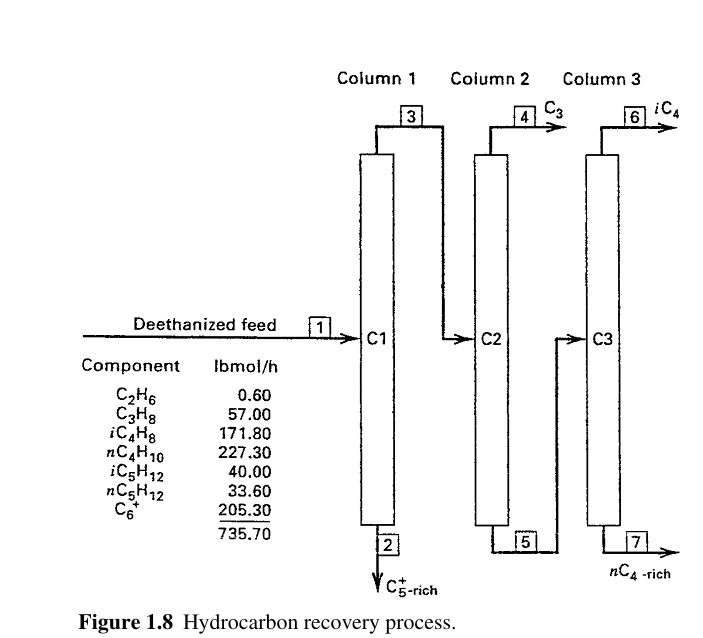
\includegraphics[width=0.8\textwidth]{FR.png}
		
		
		% División en dos columnas
		\begin{multicols}{2}
			\begin{itemize}
				\item Porcentaje de recuperación
				\setcounter{enumi}{1}
				\item [] \protect\scalebox{1.2}{\textcircled{2}} $C_5 \rightarrow \frac{233.3}{278.9} = 83.65\%$ %2
				\item [] \protect\scalebox{1.2}{\textcircled{4}} $C_3 \rightarrow \frac{54.8}{57} = 96.14\%$	%4
				\item [] \protect\scalebox{1.2}{\textcircled{6}} $i-C_4 \rightarrow \frac{162.5}{171.8} = 94.59\%$ %6
				\item [] \protect\scalebox{1.2}{\textcircled{7}} $n-C_5 \rightarrow \frac{215.8}{227.3} = 94.94\%$ %8
				\item Pureza molar del producto
				\item []$\frac{233.3}{234.1} = 99.66\% mol$
				\item []$\frac{54.8}{56} = 97.86\% mol$
				\item []$\frac{162.5}{175.5} = 92.59\% mol$
				\item []$\frac{215.8}{270} = 79.93\% mol$
			\end{itemize}
		\end{multicols}
	} % Cierre correcto de \ex{}
\end{raggedright}
\subsubsection{Fracción de separación}
\begin{raggedright}
	La fracción de separación es la relacion entre dos caudales individuales relativos al mismo compuesto para el mismo dispositivo teniendo en cuenta la corriente de salida rica en la especie mas volatil y la corriente de alimentacion.
	cuanta menor sea su volatilidad menor sera la fraccion de separacion, es decir si la fraccion de separacion es 0, los componentes estan en equilibrio. Es decir:\\
	
	\begin{equation*}
		SF =\frac{\text{Caudal molar del componente en el producto}}{\text{Caudal molar del componente en la alimentación de ese equipo}}
	\end{equation*}
	otra forma de definirlo seria:La fracción de separación es un parámetro que mide la eficiencia con la que un proceso de separación extrae un componente específico de una corriente de alimentación y lo dirige hacia una corriente de producto.
\end{raggedright}
\subsubsection{Porcentaje de recuperación}
\begin{raggedright}
    El porcentaje de recuperación es la relación entre el caudal molar del componente en la corriente de producto y el caudal molar del componente en la corriente de alimentación del proceso inicial. Se expresa como:
    \begin{equation*}
        \%PR = \frac{\text{Caudal molar del componente en el producto}}{\text{Caudal molar del componente en la alimentación de partida}} \times 100
    \end{equation*}
    Este parámetro mide la eficiencia con la que un proceso de separación extrae un componente específico de la corriente de alimentación y lo dirige hacia la corriente de producto.

    \nt{Si se refiere al mismo equipo, el porcentaje de recuperación será igual a la fracción de recuperación.}
\end{raggedright}


\subsubsection{Razón de separación}
\begin{raggedright}
	La razón de separación es la relación entre dos caudales individuales relativos al mismo compuesto ,
	\begin{equation*}
		SR = \frac{\text{Caudal molar del componente en el producto 1}}{\text{Caudal molar del componente en el producto 2}}
	\end{equation*}
	La razón de separación es un parámetro que mide la eficiencia con la que dos procesos de separación extraen un componente específico de una corriente de alimentación y lo dirigen hacia una corriente de producto.
	
	en el caso en que solo haya 2 productos se puede definir como :
	\begin{equation*}
		SR = \frac{SF}{1-SF}
	\end{equation*}
	es decir como se distribuye un compuesto entre dos corrientes de salida.
\end{raggedright}
\subsection{Pureza}
\begin{raggedright}
    Se trata de la cantidad de un componente en una corriente de salida de un separador respecto a la cantidad total de los componentes en esa misma corriente de salida.

    \begin{itemize}
        \item[] \textbf{Clave ligera (LK):} Componente designado como el más volátil. Todos los que tengan mayor volatilidad también se consideran clave ligera.
        \item[] \textbf{Clave pesada (HK):} Componente designado como el menos volátil. Todos los que tengan menor volatilidad también se consideran clave pesada.
    \end{itemize}
\end{raggedright}
	\ex{Designar el LK y HK en una corriente de 6 componentes para hidrocarburos}{
    \begin{itemize}
        \item Metano
        \item Etano 
        \item Propano $\leftarrow$ LK
        \item Butano $\leftarrow$ HK 
        \item Pentano
        \item Hexano 
    \end{itemize}
    Es decir, los componentes clave ligera serían el metano, etano y propano, mientras que los clave pesada serían el butano, pentano y hexano.
    }


\nt{\textbf{Separación nítida:}Es aquella que cumple que es superior al 0.95* el compuesto clave ligero (LK), o el 0.05 del producto pesado HK}
\subsection{Factor de separación}
\begin{raggedright}
	El factor de separacion entre dos compuestos, es la relacion entre la fraccion de separacion del componente ligero respecto al pesado, es decir:
	\begin{equation*}
		SP_{lk,hk} = \frac{SR_{LK}}{SR_{HK}}
	\end{equation*}
	Tambien se puede definir respecto a la fraccion de separacion de los componentes, es decir:
	\begin{equation*}
		SP_{lk,hk} = \frac{SF_{LK}/SF_{HK}}{(1-SF_{HK})/(1-SF_{LK})}
	\end{equation*}
	y de otra manera definiendo con concentraciones:
	\begin{equation*}
		SP_{lk,hk} = \frac{C_{LK}^1/C_{HK}^2}{C_{LK}^1/C_{HK}^2}\hspace{0.2cm} \leftrightarrow \hspace{0.2cm} SP_{lk,hk} = \frac{\large y_{\scriptscriptstyle LK}/x_{\scriptscriptstyle LK}} {\large y_{\scriptscriptstyle HK}/x_{\scriptscriptstyle HK}}
	\end{equation*}
cuanto mayor sea el factor de separacion mas viable sera la operación siendo como maximo 1 cuando se pueda separar por completo. Esto depende de los siguientes parametros:
\end{raggedright}
\begin{itemize}
	\item Cantidades relativas de ambas fases
	\item Propiedades termodinamica de los componentes y de sus propiedades de transporte y moleculares
	\item Diseño del equipo
	\item Numero de etapas y configuracion del equipo
\end{itemize}
\mlenma{Factor de separación en columna de rectificación}
{En una columna simple de rectificación, los productos ligeros irán por el destilado, es decir, la cabeza, mientras que los pesados irán por la cola, es decir, por el residuo.  

También es posible tener extracciones laterales, conocidas como corriente de sangrado, si se quieren extraer fracciones intermedias o bien una alimentación múltiple si hay varias corrientes de entrada.  

En una columna simple podemos distinguir dos zonas para una configuración óptima, divididas por la corriente de alimentación:  
\begin{itemize}
	\item \textbf{Sección de enriquecimiento} (superior o "top"), donde sale el destilado, marcada por la \textbf{LOSE} (Línea de Operación de la Sección de Enriquecimiento). 
	\item \textbf{Sección de agotamiento} (inferior), donde sale el residuo, marcada por la \textbf{LOSA} (Línea de Operación de la Sección de Agotamiento).
\end{itemize}
}

\subsection{ Denominaciones de composicion y pureza}
\begin{raggedright}
	En función del estado de agregacion se tiende a expresar de una manera las composiciones y pureza o de otra.
	\begin{itemize}
		\item $\textbf{Mezclas gaseosas:}$ $\%$ mol que es equivalente a $\%$vol o bien fracciones molares $y_i =\frac{mol_i}{m_t}$
		\item $\textbf{liquidas:}$ $\%$ peso $(\%wt)$ o bien fracciones másicas $x_i = \frac{kg_i}{kg_t}$
		\item $\textbf{Normativa/regulaciones ambientales:}$ ppm (g/L) o ppb (mg/L)
		\item $\textbf{Disoluciones acuosas:}$ molaridad
		\item $\textbf{Mezclas acuosas:}$ Concentraciones en g/L o g/mol
	\end{itemize}
\end{raggedright}
\subsection{Secuencias de separación}
\begin{raggedright}
	De todas las secuencias posibles para seleccionar la optima depende del numero de productos.\\
	En un posible caso donde existan 3 separadores y 4 productos de salida el numero de secuencias posibles es 5.\\
	para ello es importante usar la \textbf{Tecnica Heuristica} que consiste en seleccionar la secuencia que maximice el factor de separacion, es decir que separe los componentes de forma mas eficiente.
	\begin{enumerate}
		\item Al inicio de la secuencia se reitran los compuestos químicos inestables,corrosivos o quimicamente reactivos es decir aquellos que puedan suponer peligro.
		\item Los productos finales se retiran uno a uno como productos destilados de cabeza 
		\item Al principio de la secuencia se retiran los componentes de mayor porcentaje molar en la alimentación
		\item Debe hacerse la separacion mas dificil en ausencia de otros componentes.
		\item Se deja para mas adelante en la secuencia las  separaciones que producen los productos finales de mas alta pureza
		\item se  selecciona la secuencia que favore cantidades aproximadamente equimolares de cabeza y cola en cada columna.
	\end{enumerate}
	\ex{5 corrientes de productos en 3 separadores, hidrocarburos}{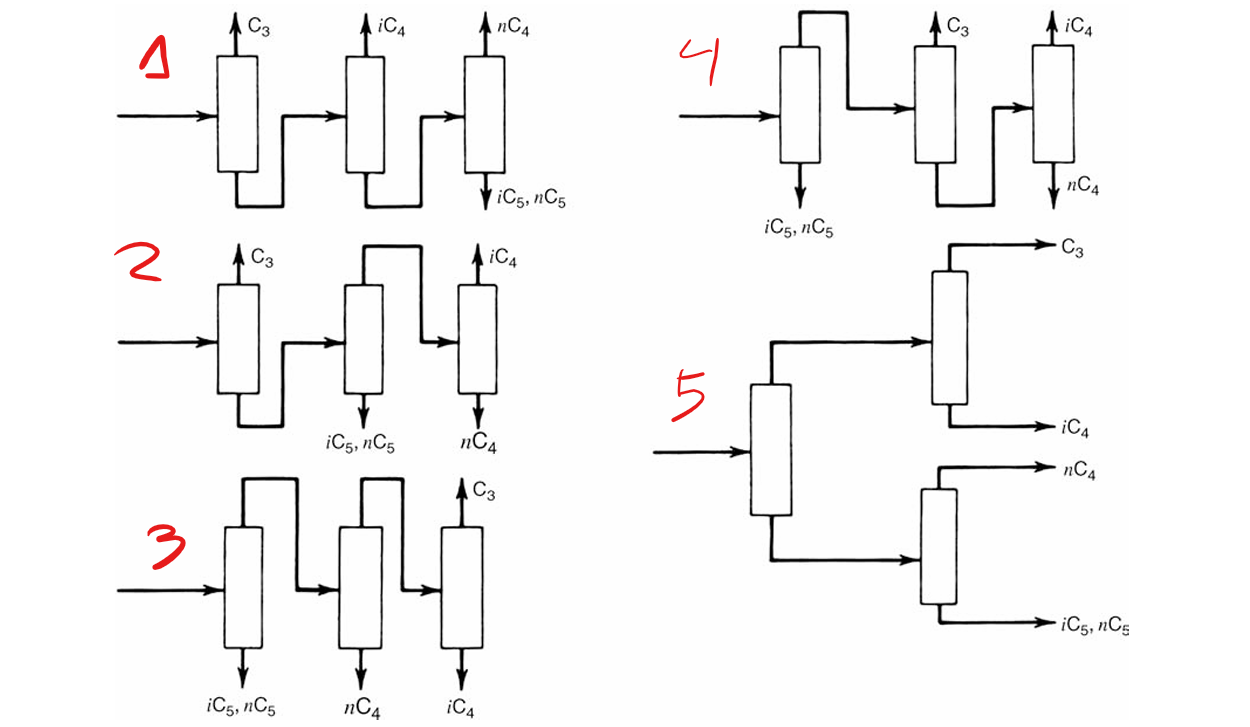
\includegraphics[width=0.7\textwidth]{Secuencias.PNG}
	\vspace{1\baselineskip}
	\begin{enumerate}
		\item como no hay ningun compuesto inestable, se pasa al siguiente paso
		\item la secuencia 1 es la que da un mayor numero de productos por cabeza
		\item en la 3 y 4 se elima los de mayor porcentaje es decir la mezcla binaria
		\item las especies que tengan volatilidades cercanas, es decir puntos de ebullicion cercano, y por tanto isomeros seran complicados de separar
		\item se desconoce la pureza de los productos, por lo que no se puede aplicar
		\item tanto la 3 como la 4 serian optimas
	\end{enumerate}
	Por tanto la seleccionada deberia ser la 4 puesto que la separacion del n-butano en la secuencia 3 es mas dificil de realizar que la del isobutano en la secuencia 4 aunque probablemente la secuencia 3 sea necesario por una extracción liquido liquido.}
\end{raggedright}
\subsection{Selección de Separaciones posibles}

\noindent\textbf{Para seleccionar una operación de separación es necesario tener en cuenta:}
\begin{enumerate}
    \item\label{n:1} \textbf{Condiciones de la alimentación}
    \begin{itemize}[label=-]
        \item Composición, en especial de las especies a separar o recuperar
        \item Caudales 
    \end{itemize}

    \item\label{n:2} \textbf{Condiciones de los productos}
    \begin{itemize}[label=-]
        \item Purezas requeridas
    \end{itemize}

    \item\label{n:3} \textbf{Aprovechamiento de las diferencias de propiedades}
    \begin{itemize}[label=-]
        \item Moleculares
        \item Termodinámicas
        \item De transporte
    \end{itemize}

    \item\label{n:4} \textbf{Características de la operación}
    \begin{itemize}[label=-]
        \item Facilidad de cambio de escala
        \item Facilidad de puesta en marcha
        \item Requerimientos de temperatura, presión y estado de agregación
    \end{itemize}

    \item\label{n:5} \textbf{Económicos}
    \begin{itemize}[label=-]
        \item Coste de la operación
        \item Coste de la inversión
    \end{itemize}
\end{enumerate}

\subsection{Questionario}
\qs{¿Cuáles son las dos operaciones clave en la ingeniería química?}{Son aquellas que modifican la composición química de la sustancia: reacciones químicas y separaciones de mezclas (de productos que están en equilibrio termodinámico)}
\qs{¿Cuáles son las principales operaciones auxiliares en la ingeniería química?}{No involucran cambios en la composición química de la sustancia, pero son necesarias para el éxito de las operaciones clave. Son separaciones de fases (de productos que no están en equilibrio termodinámico), intercambiadores de calor, bombas o compresores, mezclado o división de corrientes, aglomeración de sólidos, reducción del tamaño de sólidos y separación de sólidos por tamaño.}
\qs{\fontsize{8.55pt}{9pt}\selectfont¿Cuáles son las cinco técnicas básicas de separación y qué tienen todas ellas en común?}{
	\begin{itemize}
		\item Separación por adición de fase con un AMS
		\item Separación por creación de fase con un AES
		\item Por el uso de una barrera(membrana) que actúa en base a propiedades moleculares entre fases o sustancias relacionadas por el equilibrio termodinámico.
		\item Separación por agente sólido
		\item Separación por campo de fuerza o gradiente
	\end{itemize}
	Todas ellas tienen en común que requieren energía y que transforman una única corriente de entrada (alimentación, mezcla) en varias corrientes de salida (fases o productos que difieren en composición) por la acción del proceso de separación.
}
\qs{\fontsize{8.3pt}{10pt}\selectfont¿Por qué es la transferencia de masa un factor importante en los procesos de separación?}{La velocidad de transferencia de masa o de materia por difusión determina directamente el tamaño del equipo requerido para el proceso de separación.}
\qs{¿Qué limita el grado en que se puede lograr la separación de una mezcla?}{El aprovechamiento de las diferencias en las propiedades moleculares y/o globales o macroscópicas (termodinámicas y de transporte)}
\qs{¿Cuál es el método más común usado para separar dos fases fluidas?}{La destilación}
\qs{\fontsize{8.55pt}{9pt}\selectfont¿Cuál es la diferencia entre un AES y un AMS? Da tres desventajas de usar un AMS.}{El AMS es una sustancia que añade una nueva fase a la alimentación y se suele solubilizar mejor con uno de los componentes y de este modo lo separa del resto ( posteriormente el AMS se debe separar del componente que ha retirado); mientras que el AES provoca la generación de una nueva fase por la acción de trabajo mecánico o energía.\\
\textbf{Desventajas AMS:}
\begin{itemize}
	\item generación de pérdidas, es necesaria una separación adicional (normalmente con un AES) para separar el AMS de la sustancia retirada de la mezcla.
	\item recirculación o recuperación del AMS, para minimizar las pérdidas se debe recircular o recuperar y se deben emplear medios para ello. 
	\item Posible contaminación  del producto por el AMS, ninguna separación alcanza el 100$\%$ de éxito, luego el AMS puede impurificar el producto final que se retiró de la mezcla.
	\item Procedimientos de diseño más difíciles, las operaciones con AMS son más difíciles de diseñar que aquellas con AES.
\end{itemize}
}
\qs{¿Cuál es la operación de separación industrial más extensamente usada?}{La destilación, es la operación con mayor madurez tecnológica y de uso tiene y es la más extendida y más normalizada en cuanto a equipos, etc}
\qs{¿Cuál es la diferencia entre absorción y adsorción?}{La técnica por la que se genera la nueva fase: En la absorción, por adición de fase con un AMS (líquido absorbente) y en la adsorción, por el contacto con un agente sólido adsorbente.
\begin{itemize}
	\item La absorción se aplica a fases vapor-líquido y la adsorción a fases fluido-sólido. Por lo tanto, la interfase generada y la transferencia de materia en cada una será diferente.
\end{itemize}
}
\qs {}{El grado de separación en una operación de separación suele ser especificado en términos de recuperación de componentes y/o de purezas de productos. ¿ En qué se diferencia estos dos?}
\sol La recuperación de un componente en un aparato en el que se lleva a cabo una operación de separación se define como el caudal molar individual del componente en la corriente de salida del aparato (más rica en las especies más volátiles) entre el caudal molar individual de dicho componente en la alimentación inicial del sistema; mientras que la pureza del producto se define como el caudal molar individual del componente en la corriente de salida del aparato (más rica en las especies más volátiles) entre el caudal total que entra a dicho aparato.
\qs{¿Qué es un componente clave?}{Los componentes claves son sustancias para las cuales se diseña el dispositivo de separación con el interés de separarlas y/u obtenerlas. Normalmente se eligen dos compuestos clave; para el caso de dicha columna, si se ordenan en orden decreciente de volatilidaddes, los compuestos claves son adyacentes; el del menor punto de ebullición es llamado clave ligero y el de mayor punto de ebullición clave pesado.}
\qs{¿Qué es un producto multicomponente?}{Producto final obtenido que está formado por varias sustancias }
\section{Problemas}
\begin{raggedright}
	\textbf{Problema 01-01:} 
	Se destilan 500kmol/h de una mezcla de alcoholes, contenido 40$\% _{mol}$ de metanol, 35$\% _{mol}$ de etanol,15$\% _{mol}$ de isopropanol y 10$\% _{mol}$ de n-propanol.
		en dos columnas para su separación. El destilado de la primera columna es metanol con una pureza y recuperacion del 98$\% _{mol}$ y 96$\%$ respectivamente, 
		El destilado de la segunda columna es etanol con una pureza del 92$\%$ mol y una recuperacion del 95$\% _{mol}$ respecto de la alimentación. Asúmase la ausencia de propanoles en el destilado de la primera columna, ausencia de metanol en los residuos de la segunda y ausencia de n-propanol en el destilado de la segunda columna.
	\begin{enumerate}[label=\textbf{\alph*)}]
		\item Dibuje el diagrama de bloques del proceso numerando las columnas y corrientes. Calcule los caudales molares totales y de cada componente en todas las corrientes y construya una tabla con los resultados obtenidos.
		\item Calcule la pureza en propanoles en base molar del residuo de la segunda columna.
		\item ¿Cuál seria la maxima pureza del etanol alcanzable en el destilado de la segunda columna si se mantiene su recuperación en el 95$\%$?
		\item ¿Cuál seria la maxima recuperación (respecto de la alimentacíon) posible de etanol en el destilado de la segunda columna si su pureza se mantiene fija en el 92$\% _{mol}$? En este caso, ¿cuál seria el caudal molar total y de isopropanol en el destilado de la segunda columna?
		\item Si se mantiene la recuperación total de etanol en el destilado de la segunda columna en el 95$\%$ y la razon de separacion de isopropanol en la segunda columna fuera 0.2 (destilado respecto a residuo), ¿cuál seria la pureza del etanol en el destilado de la segunda columna?
	\end{enumerate}
\sol

	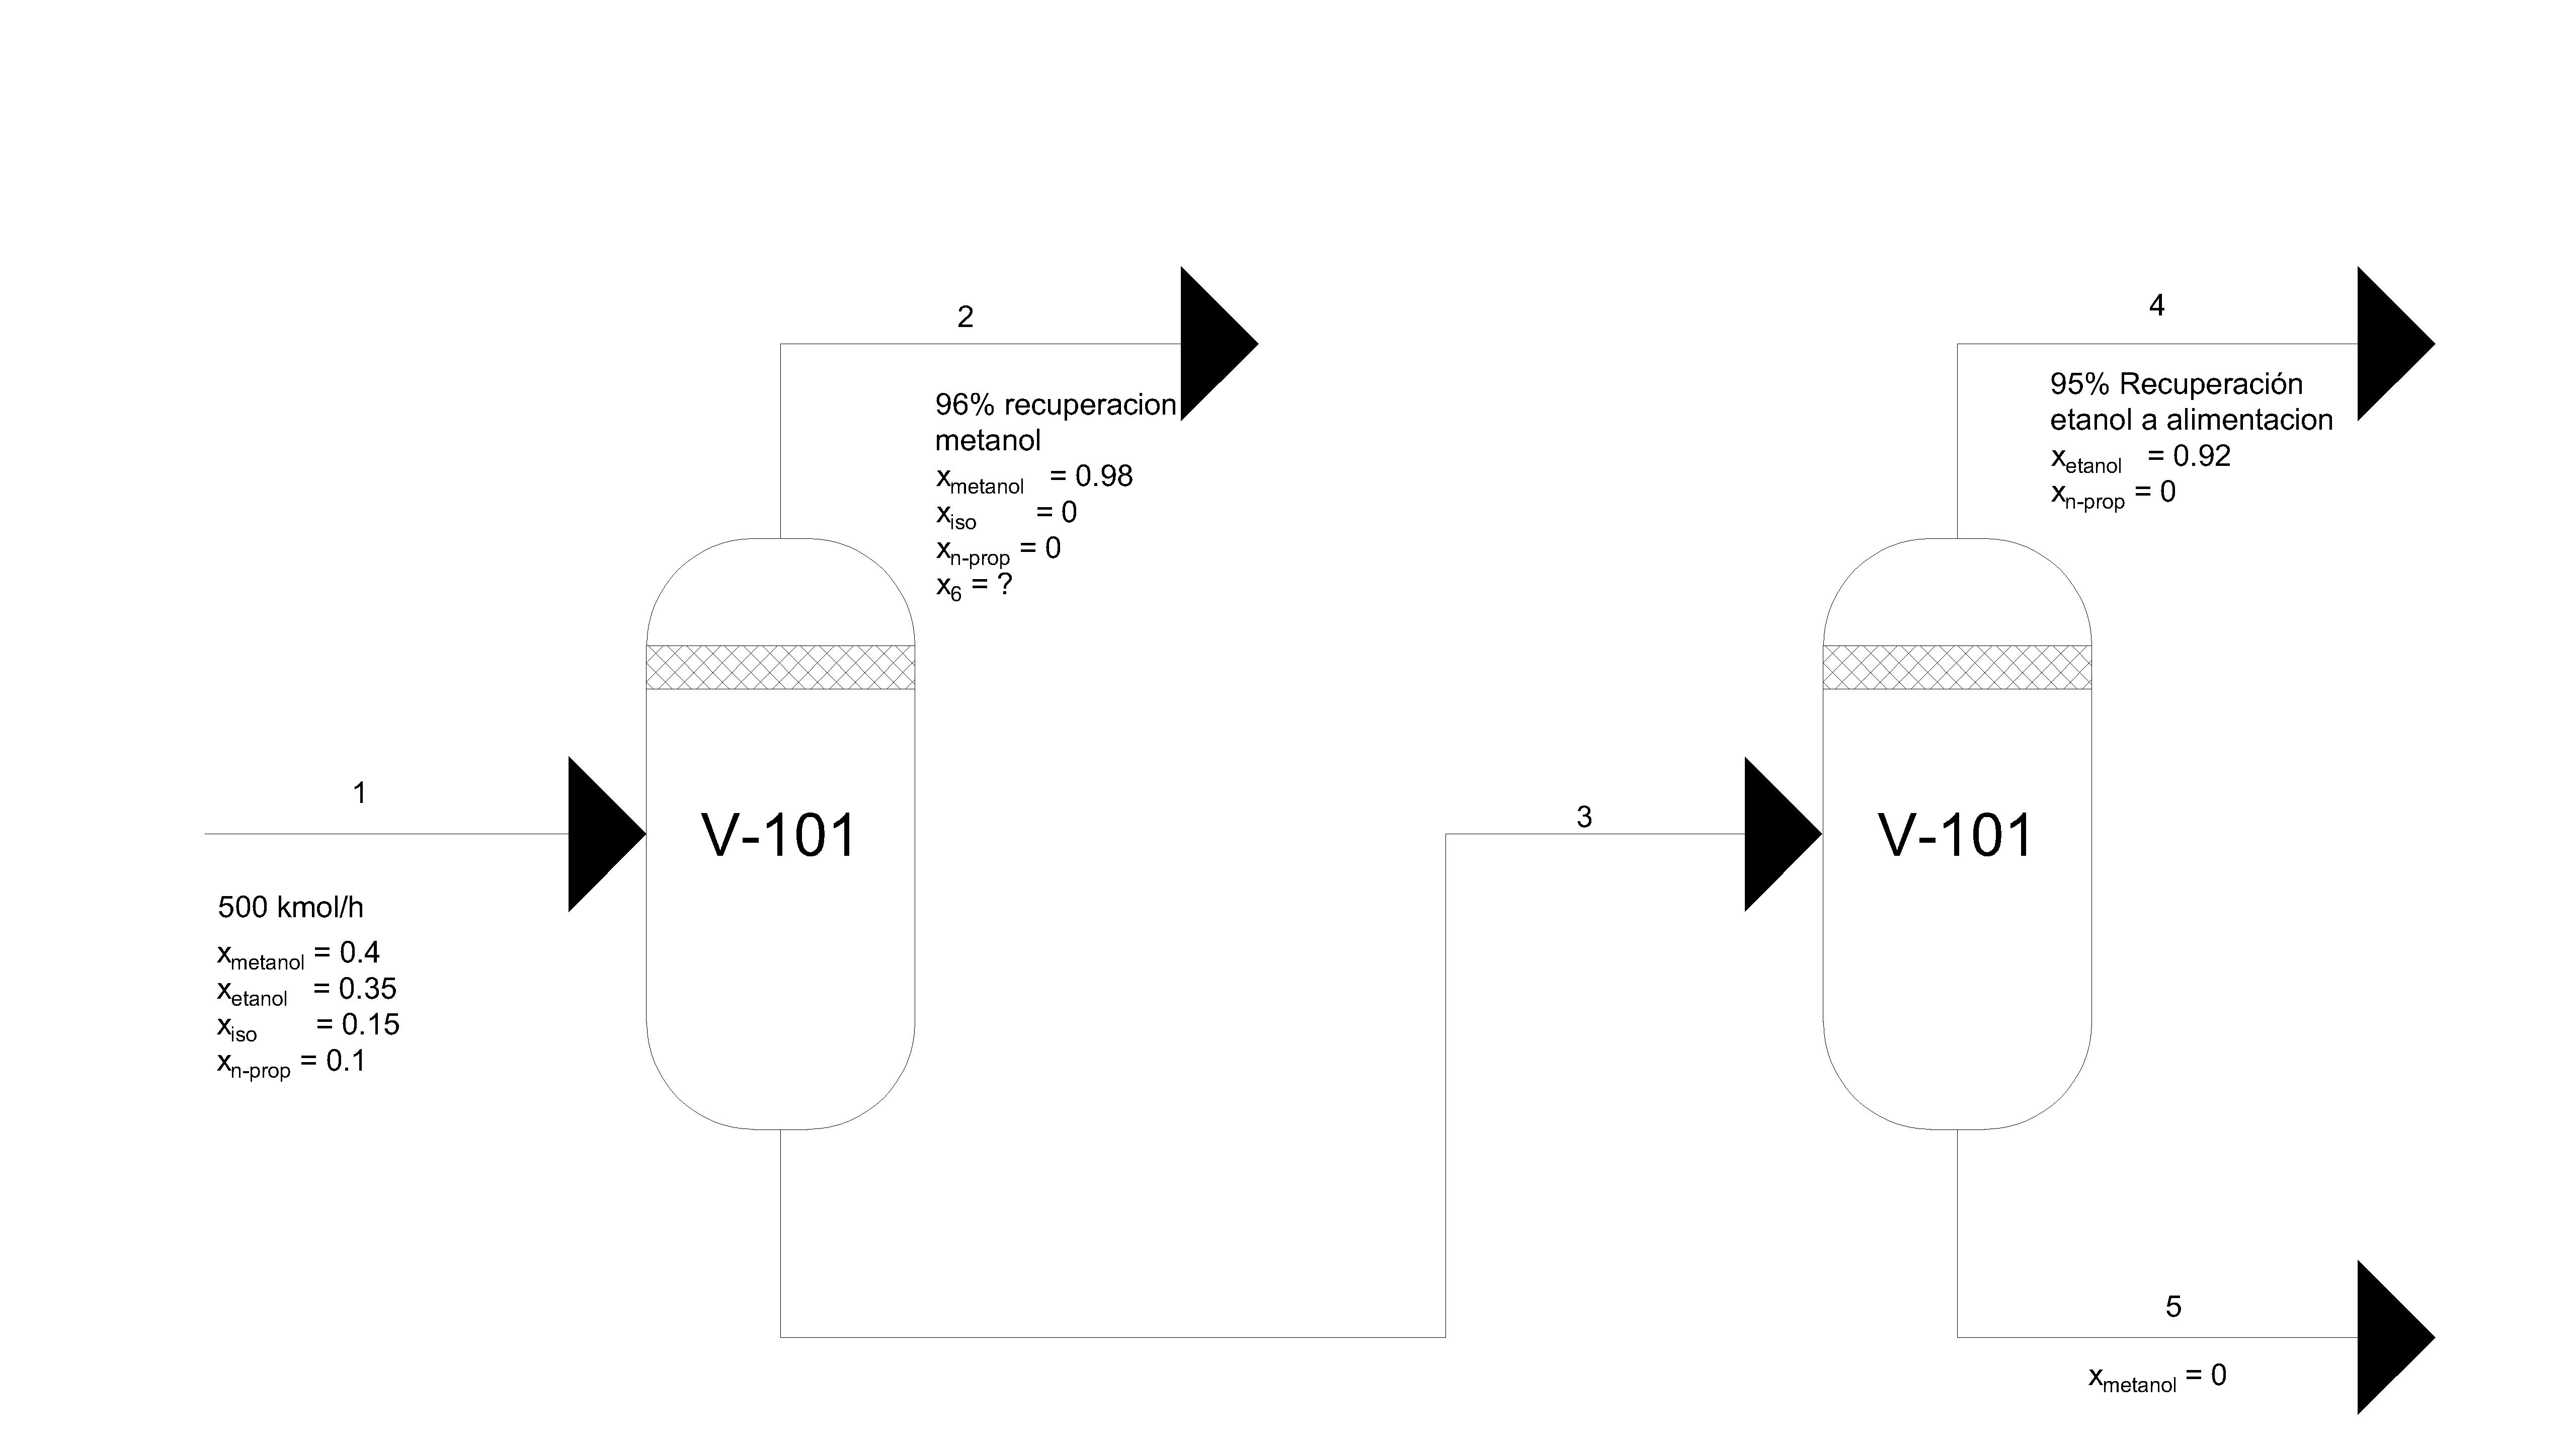
\includegraphics[width=1\textwidth]{problema1.jpg}\\
\textbf{A)}\\
\vspace{1\baselineskip}
\begin{enumerate}
	\item [] \textbf{Corriente1 :} metanol 500 $\cdot $ 0.4 = 200 kmol/h, etanol 500 $\cdot $ 0.35 = 175 kmol/h, isopropanol 500 $\cdot $ 0.15 = 75 kmol/h, n-propanol 500 $\cdot $ 0.1 = 50 kmol/h.\\
	\item [] \textbf{Corriente2 :} metanol 200 $\cdot $ 0.92 = 192 kmol/h, Recuperacion 192$\cdot$ 0.98 = 195.92 kmol/h totales $\xrightarrow[]{x_{etanol}}$ 195.92 $\cdot$ 0.02 = 3.92 kmol/h \\
	\item [] \textbf{Corriente3 :} metanol 200 $\cdot $ Caudal total = 500-195.92 = 304.08 kmol/h, BM: $\rightarrow$ 200-192 = 8 kmol/h, etanol 175-3.92 = 171.08 kmol/h, isopropanol 75 kmol/h, n-propanol 50 kmol/h.\\
	\item [] \textbf{Corriente4 :} etanol 175 $\cdot$ 0.95 = 166.25 kmol/h $\xrightarrow{x_{et}=92\%}$ $\frac{166.25}{0.92}$= 180.71 kmol/h totales
	\item [] como todo  el metanol de la corriente 3 se queda en la corriente 4, caudal de metanol = 8 kmol/h , isopropanol = 180.71 - 8 = 172.71 kmol/h.\\
	\item [] \textbf{Corriente5 :} BM total = C3-C4 = 304.08-180.71 = 123.37 kmol/h, metanol 8kmol/h , etanol 171.08 - 166.25 = 4.83 kmol/h, isopropanol 75 - 6.46 = 68.54 kmol/h, n-propanol 50 kmol/h.
\end{enumerate}
\end{raggedright}
\begin{table}[h]
    \centering
    \renewcommand{\arraystretch}{1.2}  % Aumenta el espaciado entre filas para mejor legibilidad
    \begin{tabular}{lccccc}
        \toprule
        \textbf{Corriente} & \textbf{Met (kmol/h)} & \textbf{Et (kmol/h)} & \textbf{Isoprop (kmol/h)} & \textbf{N-Prop (kmol/h)}  & \textbf{Total (kmol/h)}\\
        \midrule
        \textbf{Corriente 1} & 200 & 175 & 75 & 50 & 500\\
        \textbf{Corriente 2} & 192 & 3.92 & - & - & 195.92\\
        \textbf{Corriente 3} & 8 & 171.08 & 75 & 50 & 304.08\\
        \textbf{Corriente 4} & 8 & 166.25 & 6.46 & - & 180.71\\
        \textbf{Corriente 5} & 8 & 4.83 & 68.54 & 50 & 123.37\\
        \bottomrule
    \end{tabular}
    \caption{Caudales molares de cada corriente en kmol/h}
    \label{tabla-caudales}
\end{table}
\begin{raggedright}
\textbf{B)}\\
\vspace{1\baselineskip}
Pureza de propanoles:\\
\begin{equation*}
	P_{IP + NP} = \frac{68.54 + 50}{123.37} \cdot 100 = 100\%
\end{equation*}

\textbf{C)}\\
\vspace{1\baselineskip}
misma pureza del etanol , al recuperarse el 95$\%$ Isopropanol = 0 
\begin{equation*}
		P_{\text{et},4} = \frac{\text{kmol/h de etanol}}{\text{kmol/h totales}} = \frac{166.25}{166.25 + 8} \times 100 = 95.4\%
\end{equation*}

\end{raggedright}
\nt{Debido a que el metanol permanece en la corriente 4 y al conseguir que el isopropanol salga por 5}
\vspace{2\baselineskip}
\textbf{D)}\\

177.08 kmol/h de etanol en 4, la minima que se puede recuperar de 3 a 4 es el mismo etanol.\\
	% \begin{equation*}
	% 	177.08 \frac{\text{kmol et}}{\text{h}} \times \frac{\text{kmol total}}{0.92 \, \text{kmol et}} = 185.96 \frac{\text{kmol total}}{\text{h}}
	% \end{equation*}
	
	% \begin{equation*}
	% 	\text{Isopropanol} = 185.96 - 171.08 - 8 = 6.88 \frac{\text{kmol isopropanol}}{\text{h}}
	% \end{equation*}
	% \nt{Como se recupera mas etanol en la corriente respecto de la alimentacion (175) para mantener el 92$\%$ de recuperacion hay que modificar el caudal de entrada}
% \begin{equation*}
%     A + B + \cancelto{0}{C} = A + B
% \end{equation*}
\chapter{Transferencia de masa}

\end{document}
